感覚運動写像とは,センサー値を変数とする関数によってモーターの出力を決定することであり,その瞬間のセンサー値だけを使うと,最も単純な反応行動のための知能の一つである.
本研究では,非線形写像モデルが使われている.

1.距離デーダーの相乗平均:

\begin{equation}
  x_{\rm L} = e^{\gamma \ln d_{\rm C}} \cdot e^{(1-\gamma)\ln d_{\rm L}} 
\end{equation}
\begin{equation}
  x_{\rm R} = e^{\gamma \ln d_{\rm C}} \cdot e^{(1-\gamma)\ln d_{\rm R}} 
\end{equation}

中央のセンサーでもらった距離デーダー($d_{\rm C}$)と左のセンサーでもらった距離デーダー($d_{\rm L}$)が式(1)で計算して,左の感覚運動写像方程式の入力($x_{\rm L}$)がもらえる,同じように,真中のセンサーでもらった距離デーダー($d_{\rm R}$)と右のセンサーでもらった距離デーダー($d_{\rm R}$)が式(2)で計算して,右の感覚運動写像の入力($x_{\rm R}$)がもらえる.$\gamma$は重みであり,$\gamma$イコール0.33のとき,等加重である.

2.感覚運動写像:
\begin{equation}
\begin{aligned}
  m_{\rm R} = &\alpha \tanh(\beta_1(x_{\rm L} - b_{\rm L})) + \\
        &\alpha \tanh(\beta_2(x_{\rm L} - b_{\rm L})) + c
\end{aligned}
\end{equation}

\begin{equation}
\begin{aligned}
  m_{\rm L} = &\alpha \tanh(\beta_1(x_{\rm R} - b_{\rm R})) + \\
        &\alpha \tanh(\beta_2(x_{\rm R} - b_{\rm R})) + c
\end{aligned}
\end{equation}
式(1)と(2)でもらった$x_{\rm L}$と$x_{\rm R}$を式(3)と(4)に代入して,ロボットの右モーターの出力($m_{\rm R}$)と左モーターの出力($m_{\rm L}$)が計算できる.係数$\alpha$がロボットの最大速度を制御する,係数$\beta$が{\rm tanh}の傾きを制御する,係数$b$が関数の変曲点の位置を制御する,係数$c$が関数のだて軸上の位置を制御する. 
今回の実験のパラメーター:
$\alpha$:30;
$\beta_1$:0.004;
$\beta_2$:10;
$c$:0;
ロボットグループ1の$b_{\rm L}$とロボットグループ2の$b_{\rm R}$:160;
ロボットグループ2の$b_{\rm L}$とロボットグループ1の$b_{\rm R}$:260;
   
3.パラメーター$b$の説明:
$b_{\rm L}=260$,$b_{\rm R}=160$にすると,$b_{\rm L}=260$に対応するtanh関数の変曲点が横軸の正方向に多く移動して(図4の$B$点),$x-b$が小さくなる,方程式3により,右のモーターが左のモーターより先に速度を減少するので,ロボットが右曲がりやすいである,左曲がり易いのは逆である.
\begin{figure}[!ht]
    \centering
    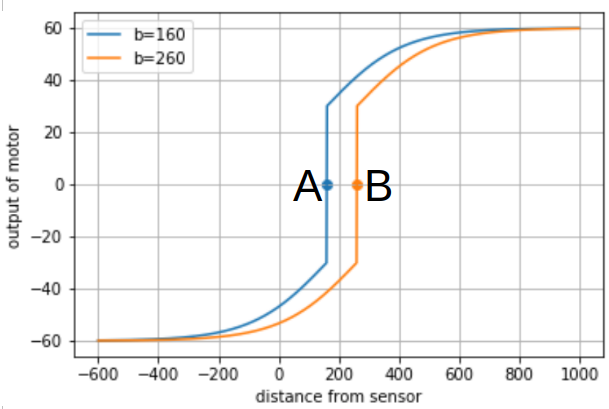
\includegraphics[width=0.7\linewidth]{tanh.jpg}
    \caption{$b=160$と$b=260$のtanh関数の曲線}
\end{figure}

